\documentclass[xcolor=dvipsnames,10pt]{beamer} %
\usepackage[utf8]{inputenc}

\usepackage{default}
\input{/home/andi/Studium/LaTex/preambel.tex}

\definecolor{dieSchoenigste}{cmyk}{
%0,.93,.67,0.08}
.77,.71,0,0
}
\mode<presentation>{\usetheme{Ilmenau}
\usecolortheme[named=dieSchoenigste]{structure}
\setbeamercovered{transparent}}


\newcommand{\Sriro}{$\mathrm{Sr}_2\mathrm{Ir}\mathrm{O}_4$\:}
\newcommand{\Lacuo}{$\mathrm{La}_2\mathrm{Cu}\mathrm{O}_4$\:}
\newcommand{\tttUmodel} {$t$-$t^{\prime}$-$t^{\prime \prime}$-$U$-model\:}




\title{Magnetic Excitations In The Iridate \Sriro}
\author{Andreas Leonhardt}
\institute{Det matematisk-naturvitenskapelige fakultet, UiO}
\date{13.06.2014}







\begin{document}
\begin{fmffile}{presi}
\fmfcmd{%
%
style_def dbl_plain_dbl_arrow expr p =
draw_double p;
shrink(1.5);
cfill (harrow (p, 0.55));
cfill (harrow (p, 0.65));
endshrink;
enddef;
%
style_def plain_dbl_arrow expr p =
draw_plain p;
shrink(1.5);
cfill (harrow (p, 0.55));
cfill (harrow (p, 0.65));
endshrink;
enddef;
%
}


 \begin{frame}
 \titlepage
 \end{frame}


\frame{\frametitle{Contents}
 			\tableofcontents}

% MODEL FRAME, containing colums, text, items and a picture
%
% \begin{frame}
%  \frametitle{Title}
% 
%   \begin{columns} 
%     \column{.5\textwidth}
%   xxx
%   \begin{itemize}
%     \item<1-> yyy
%     \item<2-> zzz
% %   \end{itemize}
% \column{.5\textwidth}
% \includegraphics[width=\textwidth]{picture.jpg}
% \end{columns} 
% \end{frame}

\section{Introduction}

\subsection{Iridates}
\begin{frame}
 \frametitle{Motivation}
 \begin{itemize}
  \item<1-> Iridates contain Iridium embedded in an oxygen complex
  \begin{center}
  \includegraphics[width=.6\textwidth]{../Periodic_table}
 \end{center}
  \item<2-> Structurally similar to the cuprates, which have Cu instead of Ir and are best know for High-Temperature Superconductivity.
  \item<3-> They provide realizations of interesting theoretical models.
 \end{itemize}
\note{
 Cuprates have been investigated since the 80's and are understood quite well but with still ongoing research  \\
 They are strongly correlated and usually described as spin systems. \\
 Similarity: chemically, crystal structure wise, d-orbitals, layout \\
 Iridates have different parameters due to their increased atomic number \\
 spin Hamiltonian still valid? \\
% Kitaev model is exactly solvable, might be useful for quantum computing\\
}
 \end{frame}

% clear definitions
\begin{frame}
 \frametitle{Open questions}
 \begin{itemize}
  \item<1-> Are there High Temperature Superconductors in the iridates?
  \item<2-> How and when does a metal-insulator transition occur?
  \item<3-> Which effective models can be used?
 \end{itemize}
 \note{
 Structurally very similar, show similar behaviour, \\
 SC proposed, but not observed. \\
 THERE IS A CONFERENCE THIS VERY WEEK WHICH DEALS WITH Fe AND Ir BASED SC. \\
 requires proper doping\\
 Due to weaker interactions closer to MIT. \\
 No complete agreement on insulating behaviour (Mott vs. Slater)\\
 Spin systems, e.g. Heisenberg? Hubbard? What are the parameters for these models?\\
 In my thesis I used the checked the Hubbard model. \\
 }
\end{frame}

\begin{frame}
 \frametitle{Goals}
 The main goals for this thesis were
 \begin{itemize}
  \item<1-> Test the Hubbard model as an effective model.
  \item<2-> Calculate the magnetic excitations of \Sriro \\ and relate them to measurements.
 \end{itemize}
\end{frame}


\subsection{\Sriro}

\begin{frame}
 \frametitle{Properties of \Sriro}
 \begin{itemize}
  \item<1-> Strong interaction between electrons
  \item<2-> Strong spin-orbit coupling (SOC)
  \item<3-> Effective spin-$\frac12$ states
  \item<4-> Antiferromagnetic ordering
  \item<5-> Weak ferromagnetic moment
  \item<6-> Insulating
 \end{itemize}
 \note{ Will explain how the later effects arise in the following slides\\
 antiferromagnet: spins are aligned antiparalell\\
 one particle per site reduces repulsion energy\\
, AF ground state, allows for virtual hopping, reducing energy further\\
 insulator due to repulsion and ordering, \\
 small ferromagnetic moment measured (mention details later)\\ 
 insulating up to Néel temperature, 240K
 }
\end{frame}


% legend for types of atoms
\begin{frame}
Building block of iridates:
\frametitle{Crystal Field}
 \begin{center}
% \tdplotsetmaincoords{0}{0}
 \begin{tikzpicture}[tdplot_main_coords]
  \node[circle,shading=ball,minimum width=.5cm,outer color=orange, inner color = white] (ball) at (0,0,0) {};
  \draw[-, ] (1,0,0) -- (0,1,0); 
  \draw[-, ] (1,0,0) -- (0,-1,0); 
  \draw[-, ] (1,0,0) -- (0,0,1); 
  \draw[-, ] (1,0,0) -- (0,0,-1); 
  \draw[-, ] (0,1,0) -- (0,0,1); 
  \draw[-, ] (0,1,0) -- (0,0,-1); 
  \draw[-, ] (0,-1,0) -- (0,0,1); 
  \draw[-, ] (0,-1,0) -- (0,0,-1); 
  \draw[-, ] (-1,0,0) -- (0,1,0); 
  \draw[-, ] (-1,0,0) -- (0,-1,0); 
  \draw[-, ] (-1,0,0) -- (0,0,1); 
  \draw[-, ] (-1,0,0) -- (0,0,-1); 
  \node[circle,shading=ball,minimum width=.3cm,color = blue, ] (ball) at (0,-1,0) {};
  \node[circle,shading=ball,minimum width=.3cm, ] (ball) at (0, 1,0) {};
  \node[circle,shading=ball,minimum width=.3cm, ] (ball) at (1,0,0) {};
  \node[circle,shading=ball,minimum width=.3cm, ] (ball) at (-1,0,0) {};
  \node[circle,shading=ball,minimum width=.3cm, ] (ball) at (0,0,1) {};
  \node[circle,shading=ball,minimum width=.3cm, ] (ball) at (0,0,-1) {};
  \draw[-, ] (1,1,1) -- (-1,1,1);
  \draw[-, ] (1,1,1) -- (1,-1,1);
  \draw[-, ] (1,1,1) -- (1,1,-1);
  \draw[-, ] (-1,-1,-1) -- (-1,-1,1);
  \draw[-, ] (-1,-1,-1) -- (1,-1,-1);
  \draw[-, ] (-1,-1,-1) -- (-1,1,-1);
  \draw[-, ] (1,-1,-1) -- (1,1,-1);
  \draw[-, ] (1,1,-1) -- (-1,1,-1);
  \draw[-, ] (-1,-1,+1) -- (-1,1,+1);
  \draw[-, ] (1,-1,+1) -- (-1,-1,+1);
  \draw[-, ] (1,-1,-1) -- (1,-1,1);
  \draw[-, ] (-1,1,-1) -- (-1,1,1);
  %
    \node[circle,shading=ball,minimum width=.5cm,outer color=orange, inner color = white] (ball) at (3,0.5,0) {};
  \node[circle,shading=ball,minimum width=.3cm, ] (ball) at (3, -.5,0) {};
  \node at (3.6,-0.5,0) {O$^{2-}$};
\node at (3.6,0.5,0) {Ir$^{4+}$};
  \end{tikzpicture}
 \end{center}
 \begin{itemize}
  \item <2-> Ligand (O$^{2-}$) field reduces rotational symmetry
  \item <3-> Lifts degeneracy of $5d$ states
 \end{itemize}

\note{
 building blocks\\
Ir embedded in octaheder of oxygen ions.\\
 creates a field with the symmetry of a cube\\
 destroys rotational symmetry\\
 split up of 5d states\\
 }
 \end{frame}

% What do I want to find out?
% Be clear about the goals and well defined
% define stuff
% are all formulas needed?
% label stuff in generally properly
% graphs:  filling bubbles
% axes
% use \stop to extend stuff
% cut out unnecessary stuff

% introducing the two types of propagators properly

% Clear Structure:
% What is it about?
% What is the problem?
% How am I going to solve it?

% connecting sentences:
% concluding the last part,
% introducing the next step.


\begin{frame}
 \frametitle{Atomic States}
 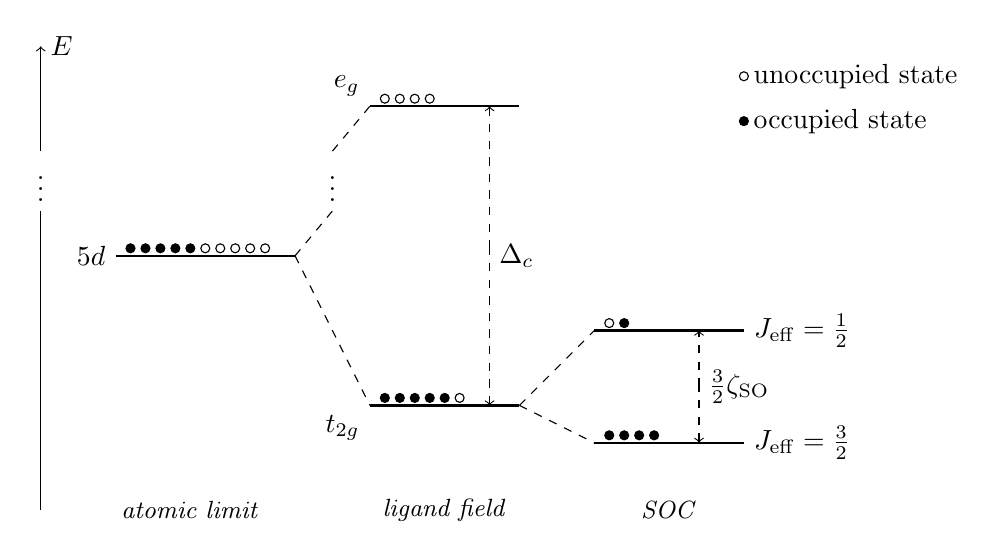
\begin{tikzpicture}[scale=1.9]
 \draw[-] (-0.7,.8) -- (-.7,2.8) node[anchor = south]{$\vdots$} ;
 \draw[->] (-0.7,3.2) -- (-.7,3.9)node[anchor =  west]{$E$};
 \draw[-,black  ,thick] (-0.2,2.5)node[anchor=east] {$5d$} -- (1.0,2.5);
 \foreach \f in {-0.1,0.0,...,0.4} \filldraw (\f,2.55) circle (0.03);
 \foreach \f in {0.4,0.5,...,0.9} \draw (\f,2.55) circle (0.03);
 %
 \draw[-,black,dashed] (1.0,2.5) -- (1.25,2.8) node[anchor= south]{$\vdots$};
 \draw[-,black,dashed] (1.25,3.2) -- (1.5,3.5);
 \draw[-,black,dashed] (1.0,2.5) -- (1.5,1.5);
 %
 \draw[-,black  ,thick] (1.5,3.5)node[anchor=south east] {$e_g$} -- (2.5,3.5);
  \foreach \f in {1.6,1.7,...,1.9} \draw (\f,3.55) circle (0.03);
 \draw[-,black  ,thick] (1.5,1.5)node[anchor=north east] {$t_{2g}$} -- (2.5,1.5);
  \foreach \f in {1.6,1.7,...,2.0} \filldraw (\f,1.55) circle (0.03);
  \draw (2.1,1.55) circle (0.03);
 %
 \draw[-,black,dashed] (2.5,1.5) -- (3,2.0);
 \draw[-,black,dashed] (2.5,1.5) -- (3,1.25);
 %
  \draw[-,black  ,thick] (3,2.0) -- (4,2.0) node[anchor= west] {$J_{\mathrm{eff}}=\frac12$} ;
  \draw (3.1,2.05) circle(0.03);
  \filldraw (3.2,2.05) circle(0.03);
 \draw[-,black  ,thick] (3,1.25) -- (4,1.25) node[anchor= west] {$J_{\mathrm{eff}}=\frac32$};
  \foreach \f in {3.1,3.2,...,3.4} \filldraw (\f,1.3) circle (0.03);
  % energie differences
  \draw[<-,black, dashed] (3.7,1.25) -- (3.7,1.625) node[anchor = west]{$\frac32\zeta_{\mathrm{SO}}$};
  \draw[->,black, dashed] (3.7,1.625) -- (3.7,2);
  %
  \draw[<-,black, dashed] (2.3,3.5) -- (2.3,2.5) node[anchor = west]{$\Delta_c$};
  \draw[<-,black, dashed] (2.3,1.5) -- (2.3,2.6);
  %
  \draw (0.3,0.8) node[]{\small{\emph{atomic limit}}};
  \draw (2.0,0.8) node[]{\small{\emph{ligand field}}};
  \draw (3.5,0.8) node[]{\small{\emph{SOC}}};
  %
  \draw (4,3.7) node[anchor = west]{unoccupied state} circle(0.03);
  \filldraw (4,3.4) node[anchor = west]{occupied state}  circle(0.03);
 \end{tikzpicture}
\note{
 scheme of the split up, not in energy scale\\
 with filling factors in the ground state\\
 crystal field splits due to reduction in symmetry\\
 $t_{2g}$ 3-fold degenerate, $e_g$ 2-fold.\\
 qualitatively, $e_g$ orbitals closer to negative oxygen ions, larger repulsion.\\
 crystal field split up is much larger than SOC\\
 $S=1/2$, $L_{eff}=1$ \\
 $J=3/2$ states completely filled\\
 left with effective spin-1/2 system\\
 half filled (w/o doping)\\
 }
 \end{frame}


% define orbital, square lattice
% clear definition
\begin{frame}
 \frametitle{Unit Cell Of \Sriro}
 \begin{center}
 \includegraphics[width=.45\textwidth]{../medium.png}
 
 Graphic taken from Jungho Kim \emph{et al.}, Phys.Rev.Lett. 108:177003.
 \end{center}
\note{
 \Sriro
 structure: layered, i.e. behaves 2D, effecitvely\\
 Main material, \Lacuo equivalent. \\
 When doped, \Lacuo is a HTSC.\\
 iridate basic building block, each layer has perovskite structure, \\
 i.e. corner sharing, but canted\\
 enlarges unit cell. Will be treated as distortion.\\
 other versions have several layers stacked on top of each other (2, $\infty$)\\
 edge sharing configurations are possible (honeycomb lattice)\\
 will treat as 2D purely. \\
 }
 \end{frame}



\begin{frame}
 \frametitle{Crystall structure of \Sriro}
 \begin{itemize}
  \item<1-> Layered
  \item<2-> 2-dimensional square lattice 
  \item<3-> One orbital, half filled 
 \end{itemize}
\end{frame}



\section[Hubbard Model]{The Hubbard Model}

\subsection{Hubbard Model}

% write description of t and U in slide
\begin{frame}
\frametitle{The Hubbard Hamiltonian}
\begin{equation*}
 H = - t \! \sum_{\langle i,j \rangle,\sigma}\! \left (c^{\dagger}_{i,\sigma}c_{j,\sigma} + c^{\dagger}_{j,\sigma}c_{i,\sigma} \right) 	 
 -\mu \sum_{i,\sigma} c^{\dagger}_{i,\sigma}c_{i,\sigma} +U \sum_i n_{i,\uparrow} n_{i,\downarrow}.
\end{equation*}
\begin{itemize}
 \item $t$: hopping term, corresponds to kinetic energy
 \item $U$: intra-orbital repulsion between electrons
 \item $n_{\sigma} = c^{\dagger}_{i,\sigma}c_{i,\sigma}$ 
 \item sum restricted to nearest neighbour pairs $\langle i,j\rangle$
 \item fermionic anti-commutation relations $\{c^{\dagger}_{i,\sigma} ,c_{j,\sigma^{\prime}}\} = \delta_{ij}\delta_{\sigma \sigma^{\prime}}; \quad 
 \{c^{\dagger}_{i,\sigma},c^{\dagger}_{j,\sigma^{\prime}} \} =0$
\item $\mu$: chemical potential
 \end{itemize}
\note{
 give Hubbard model by Hamiltonian \\
 use orthogonal atomic states (really Wannier states)\\
 t-term: kinetic term, allows for movement\\
 leads to band structure and can be measured/calculated (LDA…). (leaves U open)\\
 band structure depends on geometry.\\
 chemical potential for filling\\
 U-term: interactions. reduced to one-site interactions\\
 e.g. only electrons in the same orbital repel each other\\
 simplification, that makes the estimation of U difficult.\\
 not first principle any more.\\
 easiest model, but not solvable in 2D (solvable in 1 and $\infty$ dimensions)\\
 much used
} 
\end{frame}

\begin{frame}
\frametitle{The Hubbard Hamiltonian}
\begin{center}
  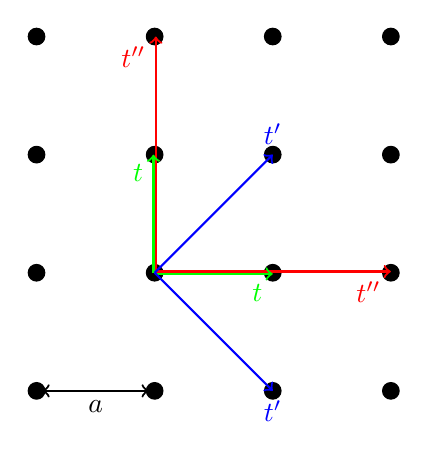
\begin{tikzpicture}[scale=1.5]
 \foreach \x in {1,...,4}
 \foreach \y in {1,...,4}
 \filldraw  (\x,\y) circle (2pt);
 \draw[->,red  ,thick] (2.01,2) -- (2.01,4) node[anchor=north east] {$t^{\prime \prime}$};
 \draw[->,red  ,thick] (2,2.01) -- (4,2.01) node[anchor=north east] {$t^{\prime \prime}$};
 \draw[->,green,thick] (1.99,2) -- (1.99,3) node[anchor=north east] {$t$};
 \draw[->,green,thick] (2,1.99) -- (3,1.99) node[anchor=north east] {$t$};
 \draw[->,blue ,thick] (2,2) -- (3,3) node[anchor= south] {$t^{\prime}$};
 \draw[->,blue ,thick] (2,2) -- (3,1) node[anchor=north ] {$t^{\prime}$}; 
 \draw[<->,thick] (1.05,1)  -- (1.95,1);
 \draw (1.5,1) node[anchor = north]{$a$};
 \end{tikzpicture}
\end{center}
\note{
First(green), second(blue) and third(red) neighbour interactions\\
non-neglible \\
similar terms as before \\
}
\end{frame}

\begin{frame}
 \frametitle{Momentum space for a square lattice}
 \begin{itemize}
  \item<1-> Periodic system $\Rightarrow k_i + \frac{2\pi}{a} \sim k_i$.
  \item<2-> Momenta restricted to Brillouin zone $[-\frac{\pi}a,\frac{\pi}a]^2$.
  \item<3-> Normalize lattice constant $a$ to 1.
  \item<4-> Finite systems with $N$ lattice sites result in $N$ discretized momenta.
 \end{itemize}
 \note{
 Repetition from solid state physics\\
 Periodic momenta, restricted to $-\pi,\pi$\\
 Discretized momenta in finite systems\\
 $N$ in total\\
 }
\end{frame}


\begin{frame}
\frametitle{The Hubbard Hamiltonian in momentum space}
 \begin{equation*}
  \hat{H} = \sum_{\vec{k},\sigma} \left(\varepsilon_{\vec k} - \mu\right) c^{\dagger}_{\vec{k},\sigma}c_{\vec{k},\sigma} + \frac{U}{N} \sum_{\vec{k}\vec{k}^{\prime}\vec{q}}
	c^{\dagger}_{\vec{k},\uparrow}c_{\vec{k}-\vec{q},\uparrow} c^{\dagger}_{\vec{k}^{\prime},\downarrow}c_{\vec{k}^{\prime}+\vec{q},\downarrow}
 \end{equation*} 
with the dispersion
\onslide<2->
\begin{equation*}
 \varepsilon_{\vec k} = -2t\left( \cos k_x + \cos k_y \right) \onslide<3-> -4t^{\prime} \cos k_x \cos k_y  -2t^{\prime \prime} \left( \cos 2k_x + \cos 2k_y \right)
\end{equation*}
\note{
 in momentum space:\\
 kinetic energy becomes diagonal, dispersion\\
 can include further neighbour interactions, changes only dispersion\\
 U term is non-diagonal. Momentum conserving
}
\end{frame}


% ================================================================================================================
% Heisenberg models

% introduce spin models properly before comparing
\begin{frame}
 \frametitle{Heisenberg model}
 \begin{itemize}
  \item<1-> Stationary spins without a kinetic term.
  \item<2-> Heisenberg Hamiltonian
  \only<2>{  \begin{equation*}H = J \sum_{\langle i,j\rangle} \vec S_i \vec S_j  
   \: \:\phantom{
   +J^{\prime} \!\!\sum_{\langle\langle i,j\rangle\rangle}\!\! \vec S_i \vec S_j
	+J^{\prime \prime} \!\! \!\!\sum_{\langle \langle\langle i,j\rangle \rangle\rangle} \!\!\!\! \vec S_i \vec S_j 
	}
  \end{equation*}}
    \item<3-> Can be derived from the Hubbard model in the large $U$ limit.
  \only<4-5>{  \begin{equation*} 
  H = J \sum_{\langle i,j\rangle} \vec S_i \vec S_j  
      +J^{\prime} \!\!\sum_{\langle\langle i,j\rangle\rangle}\!\! \vec S_i \vec S_j
	+J^{\prime \prime} \!\!\!\!\sum_{\langle \langle\langle i,j\rangle \rangle\rangle}\!\!\!\! \vec S_i \vec S_j
      \end{equation*}}
      \item<5-> $J \longrightarrow 4\frac{t^2}U,  \qquad (\frac tU\rightarrow 0)$
      \item<6-> Long range correlations become more important for lower $U$.
 \end{itemize}
 \note{
 Large $U$ prevents double occupancy, leads to stationary spins at half filling \\
 Down-folding, i.e. projection to states w/o double occupancy
 Couplings arise from virtual hoppings\\
 Coupling $J$ \\
 }
\end{frame}





\subsection{Mean Field Equations} % or Mean Field Treatement?


% conceptual
\begin{frame}
 \frametitle{Mean Field Equations}
 \begin{itemize}
  \item<1-> neglect fluctuations
  \item<2-> each particle sees only the averaged field created by all particles
  \item<3-> reduce interaction to one-particle operator
  \end{itemize}
 \only<4> { \begin{IEEEeqnarray*} {rCl}
	      U \sum_i n_{i,\uparrow} n_{i,\downarrow} &=& U \sum_i (n_{i,\uparrow}-\langle n_{i,\uparrow} \rangle ) (n_{i,\downarrow}-\langle n_{i,\downarrow} \rangle) 
	      \nonumber \\&&
	      + n_{i,\uparrow} \langle n_{i,\downarrow}\rangle + n_{i,\downarrow} \langle n_{i,\uparrow} \rangle -\langle n_{i,\uparrow} \rangle \langle n_{i,\downarrow} \rangle          
        \end{IEEEeqnarray*}}
 \only<5->{ \begin{IEEEeqnarray*} {rCl}
	      U \sum_i n_{i,\uparrow} n_{i,\downarrow} 
	       &\approx& U \sum_{i} n_{i,\uparrow} \langle n_{i,\downarrow}\rangle + n_{i,\downarrow} \langle n_{i,\uparrow}\rangle +\mathrm{const.} \\
	       &&\phantom{+ n_{i,\uparrow} \langle n_{i,\downarrow}\rangle + n_{i,\downarrow} \langle n_{i,\uparrow} \rangle -\langle n_{i,\uparrow} \rangle \langle n_{i,\downarrow} \rangle}
        \end{IEEEeqnarray*}}
 \note{
 rewrite the two-particle operator as product of two one particle operators \\
 neglect fluctuations around the mean value \\
 get one particle operators, that get a system dependent pre-factor\\
 needs to be calculated self-consistently \\
 expectation value corresponds to the field created by all other particles \\
 of opposite spin due to the form of the interaction.\\
 Left with one particle operator\\
 }
 \end{frame}

\begin{frame}
 \frametitle{Mean field equations}
 \begin{itemize}
         \item<1-> in momentum space: \\ $ \frac UN \sum_{\vec q} \sum_{\vec k, \vec k^{\prime}, \sigma}  c^{\dagger}_{\vec k + \vec q, \sigma} 
					    c_{\vec k, \sigma} \langle c^{\dagger}_{\vec k^{\prime} - \vec q, \sigma} c_{\vec k^{\prime}, \sigma} \rangle $
 \item<2-> uniform repulsion for $\vec q = 0$, $\frac1N \sum_i \langle c^{\dagger}_{\vec k,\sigma} c_{\vec k, \sigma} \rangle= n_{\sigma} $
   \item<3-> staggered magnetic field for $\vec q = \vec Q \equiv (\pi,\pi)$.  
   $\frac1N\sum_{\vec k} \langle c^{\dagger}_{\vec k, \sigma} c_{\vec k+\vec Q, \sigma} \rangle
   = \frac1N\sum_i \langle (-1)^i c^{\dagger}_{i,\sigma}c_{i,\sigma} \rangle 
   = \frac{s_{\sigma}}2 m_s \ne 0$
 \end{itemize}
 \note{
 Use same system in momentum space \\
 Have 2 contributions \\
 Particle density and its uniform repulsion, diagonal term\\
 Staggered Magnetization, alternating spin alignment. \\
 Draw picture on blackboard \\ 
 measures ordering of an AF state \\
 }
\end{frame}
 
 

\begin{frame}
\frametitle{Propagators}
 \begin{IEEEeqnarray*}{rClCc}
 G_{\vec k}(\tau) &=& \langle c_{\vec k         ,\sigma}(\tau)  c^{\dagger}_{\vec k ,\sigma}(0) \rangle &=&  
 \scalebox{.5}{\parbox{40mm}{
	      \begin{fmfgraph}(40mm,20mm)
		\fmfleft{i1}
		\fmfright{o1}
		\fmf{plain_arrow}{i1,o1}
	      \end{fmfgraph}}} \\
 F_{\vec k}(\tau) &=& \langle c_{\vec k +\vec{Q},\sigma}(\tau)  c^{\dagger}_{\vec k ,\sigma}(0) \rangle 
 &=&
 \scalebox{.5}{\parbox{40mm}{
	      \begin{fmfgraph}(40mm,20mm)
		\fmfleft{i1}
		\fmfright{o1}
		\fmf{plain_dbl_arrow}{i1,o1}
	      \end{fmfgraph}}}
\end{IEEEeqnarray*}
\note{
creates two non-zero propagators \\
diagonal term, including, band structure, chemical potential, uniform density \\
off-diagonal term \\
proportional to ordering and repulsion \\
}
\end{frame}



\begin{frame}
 \frametitle{Mean Field Propagators}
 Self consistent Dyson equation \\
 Coupled differential equation that can be solved analytically
  \begin{center}
 \begin{IEEEeqnarray*}{rCl}
%\vcenter{ \hbox{
 \scalebox{.5}{\parbox{40mm}{
	      \begin{fmfgraph}(40mm,40mm)
		\fmfleft{i1}
		\fmfright{o1}
		\fmf{dbl_plain_arrow}{i1,o1}
	      \end{fmfgraph}}}
&=& \scalebox{.5}{\parbox[][][t]{30mm}{\begin{fmfgraph}(30mm,40mm) \fmfleft{i} \fmfright{o} \fmf{plain_arrow}{i,o} \end{fmfgraph}} }
   + \scalebox{.5}{\parbox{50mm}{\begin{fmfgraph}(50mm,40mm) \fmfleft{i1} \fmfright{o1} \fmf{plain_arrow}{i1,v1} \fmf{dbl_plain_dbl_arrow}{v1,o1}
					   \fmf{dashes,tension=0}{v2,v1} 	 \fmfforce{0.5w,.8h}{v2}     \fmf{dbl_plain_dbl_arrow,tension=0.7}{v2,v2}
                \end{fmfgraph}}}
	+   \scalebox{.5}{ \parbox{50mm}{\begin{fmfgraph}(50mm,40mm) \fmfleft{i1} \fmfright{o1} \fmf{plain_arrow}{i1,v1} \fmf{dbl_plain_arrow}{v1,o1}
					   \fmf{dashes,tension=0}{v2,v1} 	 \fmfforce{0.5w,.8h}{v2}     \fmf{dbl_plain_arrow,tension=0.7}{v2,v2} \end{fmfgraph}}}
 \end{IEEEeqnarray*}
 \begin{IEEEeqnarray*}{rCl}
 \scalebox{.5}{\parbox{40mm}{
	      \begin{fmfgraph}(40mm,40mm)
		\fmfleft{i1}
		\fmfright{o1}
		\fmf{dbl_plain_dbl_arrow}{i1,o1}
	      \end{fmfgraph}}}
&=& \scalebox{.5}{\parbox{50mm}{\begin{fmfgraph}(50mm,40mm) \fmfleft{i1} \fmfright{o1} \fmf{dbl_plain_dbl_arrow}{i1,v1} \fmf{plain_arrow}{v1,o1}
					   \fmf{dashes,tension=0}{v2,v1} 	 \fmfforce{0.5w,.8h}{v2}     \fmf{dbl_plain_arrow,tension=0.7}{v2,v2}
                \end{fmfgraph}}}
	+    \scalebox{.5}{\parbox{50mm}{\begin{fmfgraph}(50mm,40mm) \fmfleft{i1} \fmfright{o1} \fmf{plain_arrow}{i1,v1} \fmf{dbl_plain_arrow}{v1,o1}
					   \fmf{dashes,tension=0}{v2,v1} 	 \fmfforce{0.5w,.8h}{v2}     \fmf{dbl_plain_dbl_arrow,tension=0.7}{v2,v2} \end{fmfgraph}}}
\end{IEEEeqnarray*} 
\end{center}
\end{frame}


% which diagrams are neglected?
% and why?

% propagators

\begin{frame}
\frametitle{Propagators}
\begin{IEEEeqnarray*}{rCl}
 G_{\vec k ,\sigma}(\im \omega_n) &=& \frac{ \im \omega_n - \varepsilon_{\vec k +\vec{Q}} +\mu -Un_{-\sigma} }
					    { (\im \omega_n - E_{\vec k ,\sigma}^+) (\im \omega_n - E_{\vec k ,\sigma}^-) },
\\
 F_{\vec k ,\sigma}(\im \omega_n) &=& \frac{ Um_{s,-\sigma} }
					    { (\im \omega_n - E_{\vec k ,\sigma}^+) (\im \omega_n - E_{\vec k ,\sigma}^-)}.
\end{IEEEeqnarray*}
with the poles located at
\begin{equation*}
 E^{\pm}_{\vec k, \sigma} = \frac{\varepsilon_{\vec k }+\varepsilon_{\vec k +\vec{Q}}}2 -\mu + Un_{-\sigma}  \pm \sqrt{ \left(\frac{\varepsilon_{\vec k }-\varepsilon_{\vec k +\vec{Q}}}2\right)^2 + U^2m_{s,-\sigma}^2 }
\end{equation*}
\end{frame}


\begin{frame}
 \frametitle{Energy bands $E^{\pm}_{\vec k,\sigma}$}
 \begin{center}
  \includegraphics[width=.4\textwidth]{../EpEm_tttU44}
 \end{center}
 Dispersion for the \tttUmodel.
 \begin{itemize}
  \item<2-> The $J_{\mathrm{eff}} = \frac12$- band is split due to the interaction.
  \item<3-> Explains insulating state.
  \item<4-> Symmetric under translations of $\vec Q = (\pi,\pi)$.
 \end{itemize}
\end{frame}



% non-diagonal propagator and AF ground state
% staggered magnetization and $\vec Q$. 
% show staggered magnetization here
\begin{frame}
 \frametitle{Staggered magnetization}
 \begin{center}
  \includegraphics[width=.6\textwidth]{../stagmag_T10.png} \\
 Staggered magnetization as function of $\frac Ut$
 \end{center}
\end{frame}


\subsection{Dynamic Magnetic Susceptibility}



\begin{frame}
 \frametitle{Excitations}
 \begin{itemize}
  \item<1-> study basic magnetic excitations by inelastic scattering: \\ neutron or X-ray (RIXS).
  \item<2-> Differential scattering cross section directly related to dynamic magnetic susceptibility.
  \item<3-> Poles at basic excitations of the system.
  \item<4-> transferred energy and momentum  give magnon dispersion.
  \item<5-> Dynamical magnetic susceptibility is a two-point correlation function,
   \begin{equation*}
  \chi^{+-}(\tau,\vec q) = \sum_{\vec k \vec k^{\prime}} \langle c^{\dagger}_{\vec k+\vec q, \uparrow}\!(\tau)\: c_{\vec k, \downarrow}\!(\tau)\: 
		      c^{\dagger}_{\vec k^{\prime}, \downarrow}\!(0)\: c_{\vec k^{\prime}+\vec q, \uparrow}\!(0)\: \rangle
 \end{equation*}
 \item<6-> Can be expressed in terms of propagators.
 \end{itemize}
 \note{
 two point correlation function, response function \\
 longitudinal and transversal susceptibility \\
 link to scattering cross section, meaning and importance of poles\\
 $\omega(\vec q)$ from pole structure\\
 basic excitations of spin waves <--- Definition and ILLUSTRATION of SWs\\
  $\frac{\dint^2 \sigma}{\dint \omega \dint \Omega} = -2\Im \chi(\omega, \vec q) $\\
  }
\end{frame}


% diagrammatic expansion
\begin{frame}
 \frametitle{Diagrammatic Expansion}
 \begin{IEEEeqnarray*}{rCl}
  \chi^{+-} &=& 
 \scalebox{.5}{ \parbox{60pt}{ \begin{fmfgraph*}(60,50)
  \fmfleft{i1} \fmfright{o1}  \fmf{dbl_plain_arrow,left=.55}{i1,o1} \fmf{dbl_plain_arrow,left=.55}{o1,i1}
  \fmfdot{i1,o1}
 \end{fmfgraph*}}}
 \:+\: 
 \scalebox{.5}{\parbox{100pt}{  \begin{fmfgraph*}(100,50)
  \fmfleft{i1} \fmfright{o1}  \fmf{dbl_plain_arrow,left=.25}{i1,v1,o1} \fmf{dbl_plain_arrow,left=.25}{o1,v2,i1} \fmf{dashes, tension=0}{v1,v2}
  \fmfforce{.5w,h}{v1} \fmfforce{.5w,0}{v2}
    \fmfdot{i1,o1}
 \end{fmfgraph*}}} %\nonumber \\[.5cm] &&
 + \:  
 \scalebox{.5}{\parbox{180pt}{\begin{fmfgraph*}(180,50)
  \fmfleft{i1} \fmfright{o1}  
  \fmf{dbl_plain_arrow,left=0.25}{i1,v1} \fmf{dbl_plain_arrow,left=.0}{v1,v3} \fmf{dbl_plain_arrow,left=.25}{v3,o1} 
  \fmf{dbl_plain_arrow,left=.25}{o1,v4} \fmf{dbl_plain_arrow,left=.0}{v4,v2} \fmf{dbl_plain_arrow,left=.25}{v2,i1} 
  \fmf{dashes, tension=0.0}{v1,v2} \fmf{dashes, tension=.0}{v3,v4}
  \fmfforce{.33w,h}{v1} \fmfforce{.33w,0}{v2} \fmfforce{.66w,h}{v3} \fmfforce{.66w,0}{v4}
   \fmfdot{i1,o1}
\end{fmfgraph*}}}
 \:+\: \cdots
 \nonumber \\[1.5cm]
 %
 %
 \chi^{zz} &=&
 \scalebox{.5}{\parbox{40pt}{\begin{fmfgraph*}(40,50)
 \fmfleft{i1} \fmfright{o1}
 \fmf{dbl_plain_arrow,left=1.00}{i1,o1} \fmf{dbl_plain_arrow,left=1.00}{o1,i1}
 \fmfdot{i1,o1}
 \end{fmfgraph*}}}
 \:+\:
 \scalebox{.5}{ \parbox{120pt}{\begin{fmfgraph*}(120,50)
 \fmfleft{i1} \fmfright{o1}
 \fmf{dbl_plain_arrow,left=1.00}{i1,v1} \fmf{dbl_plain_arrow,left=1.00}{v1,i1}
 \fmf{dashes,tension=2.5}{v1,v2} \fmf{dbl_plain_arrow,left=1.00}{v2,o1} \fmf{dbl_plain_arrow,left=1.00}{o1,v2}
 \fmfdot{i1,o1}
\end{fmfgraph*}}}
 \:+\:
 \scalebox{.5}{ \parbox{180pt}{\begin{fmfgraph*}(180,50)
 \fmfleft{i1} \fmfright{o1}
 \fmf{dbl_plain_arrow,left=1.00}{i1,v1} \fmf{dbl_plain_arrow,left=1.00}{v1,i1}
 \fmf{dashes,tension=2.5}{v1,v2} 
 \fmf{dbl_plain_arrow,left=1.00}{v2,v3} \fmf{dbl_plain_arrow,left=1.00}{v3,v2}
 \fmf{dashes,tension=2.5}{v3,v4} 
 \fmf{dbl_plain_arrow,left=1.00}{v4,o1} \fmf{dbl_plain_arrow,left=1.00}{o1,v4}
 \fmfdot{i1,o1}
\end{fmfgraph*}}} 
\:+\: \cdots\nonumber
 \end{IEEEeqnarray*}
\end{frame}





% RPA, non-crossing approximation
% geometric sum, analytical expression
% quantum corrections? mention with RPA, that a rescaling needs to be included later. 
\begin{frame}
 \frametitle{Random Phase Approximation}
 \begin{itemize}
  \item<1-> Sum subclass of diagrams to infinite order.
  \item<2-> Yields a closed form expression.
  \item<3-> no UV divergence due to periodicity, \\ IR divergences are possible in infinite systems.
  \item<4-> Neglecting quantum fluctuations requires rescaling of energies. 
 \end{itemize}

\end{frame}

% analytical continuation (rather not mentioning it in detail)


\section{Results}

\begin{frame}
 \frametitle{Specifications}
 \begin{itemize}
  \item Band structure given
  \item $U$ as only adjustable parameter
  \item calculate dispersion along symmetry lines of dispersion
 \end{itemize}
 \end{frame}
 
 \begin{frame}
 \frametitle{Brillouin zone}
 % =============================================================================================
 % change label to q_x and q_y
 % =============================================================================================
\begin{center}
 \includegraphics[width=.7\textwidth]{../path}
\end{center}
\end{frame}

% limit, rerun plot in order to get a nices labeling. Or remove numbers by hand.
\begin{frame}
 \frametitle{Large U limit}
 \begin{center}
  \includegraphics[width=.5\textwidth]{../U40} \\
  \small{$U=40t$} $\omega(\vec q) = 4\frac{t^2}U \sqrt{1-\frac12(\cos q_x + \cos q_y)}$.
 \end{center}
\end{frame}



\subsection{t-U-Hubbard Model}
% t-U-model
\begin{frame}
 \frametitle{Results for the t-U-Model}
 \begin{center}
  \includegraphics[width=.7\textwidth]{../compare_t47} \\
 Spin wave dispersion for the $t$-$U$-model with $U=4.7t$
\end{center}
 \end{frame}
% not capable of explaining everything
% why even showing it? 
 
 \subsection{t-t'-t''-U-Hubbard Model} %$t$-$t^{\prime}$-$t^{\prime \prime}$-$U$-
% t-t'-t''-U-model 
 \begin{frame}
 \frametitle{Results for the t-t'-t''-U-Model}
 \begin{center}
  \includegraphics[width=.7\textwidth]{../tttU44c} \\
 Spin wave dispersion for the $t$-$t^{\prime}$-$t^{\prime \prime}$-$U$-model with $U=4.4t$
\end{center}
 \end{frame}

 
 \begin{frame}
  \frametitle{Continuous excitations}
%\begin{figure}
 \begin{center}
% \begin{subfigure}{0.49\linewidth}
  \includegraphics[width=.4\textwidth]{../fuck}
%  \caption{calculated spin wave dispersion for $U=4.4$.}
%  \label{tttU44_longw}
% \end{subfigure}
%\begin{subfigure}{.49\linewidth}
 \includegraphics[width=.4\textwidth]{../measuredexit}
% \caption{measured excitations, \\taken from \cite{PhysRevLett.108.177003} }
% \label{experimental_longw}
%\end{subfigure}
%\caption{comparison of the excitation spectrum  form our calculations and RIXS measurements. The energy scale in both graphs is given in eV. 
%	  The measured excitations contain also spin orbit excitations between 0.4eV and 0.8eV}
%\label{continuum}	  
%\end{figure}}
\end{center}
 \end{frame}
\subsection{}


% how did we find the U
 \begin{frame}
  \frametitle{Magnetization}
  \begin{itemize}
   \item $U=4.4t=1.1$eV
   \item just above the Metal insulator transition point for a SOC with $\zeta_{\mathrm{SO}} = 0.37$eV
   \item $m_s=0.73$
   \item charge gap $\Delta_{\mathrm{Mott}} = \max( E^+_{\vec k} - E^-_{\vec k^{\prime}}) =0.47\mathrm{eV}$ \\ (experimentally 0.54eV)
   % with quantum corrections: .54 = 1.18*4.6eV
  \end{itemize}
 \end{frame}
 
\begin{frame}
 \frametitle{Ferromagnetic moment}
\begin{itemize}
 \item Created by canted structure \\
 \begin{center}
   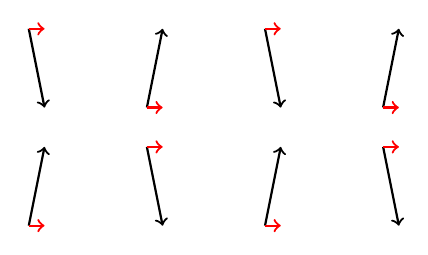
\begin{tikzpicture}
   \draw[->,thick] (-0.1,0) -- (+0.1,1);
   \draw[->,red,thick] (-0.1,0) -- (+0.1,0);
   \draw[<-,thick] (1.6,0) -- (1.4,1);
   \draw[->,red,thick] (1.4,1) -- (+1.6,1);
   \draw[->,thick] (2.9,0) -- (3.1,1);
   \draw[->,red,thick] (2.9,0) -- (3.1,0);
   \draw[<-,thick] (4.6,0) -- (4.4,1);
   \draw[->,red,thick] (4.4,1) -- (4.6,1);
  %
   \draw[<-,thick] (+0.1,1.5) -- (-0.1,2.5);
   \draw[->,red,thick] (-0.1,2.5) -- (+0.1,2.5);
   \draw[->,thick] (1.4,1.5) -- (1.6,2.5);
   \draw[->,red,thick] (1.4,1.5) -- (1.6,1.5);
   \draw[<-,thick] (3.1,1.5) -- (2.9,2.5);
   \draw[->,red,thick] (2.9,2.5) -- (3.1,2.5);
   \draw[->,thick] (4.4,1.5) -- (4.6,2.5);
   \draw[->,red,thick] (4.4,1.5) -- (4.6,1.5);
   \end{tikzpicture}
 \end{center}
 \item $\frac{M}{M_{\mathrm{local}}} = m_s \sin \Theta = 0.139$
 \item experimentally $M = 1.14\mu_b$ 
 \item $M_{\mathrm{local}} = 1\frac{\mu_b}{\mathrm{Ir}^{4+}}$, as in the  atomic limit
\end{itemize}
\end{frame}


 
 
 
% limiting case, comparison to Heisenberg and linear spin waves
% t-t'-t''-U-Hubbard model results
% t-U-Hubbard model?
% point out the meaning of the result. 

%implications
% U=4.4 =1.1eV
% insulator type?

\subsection{Further Prospects/ Outlook}

% improvements
\begin{frame}
 \frametitle{Improvements}
 \begin{itemize}
  \item Quantum corrections
  \item Refine Band structure
 \end{itemize}
\end{frame}

 \begin{frame}
 \frametitle{Further Calculations}
 \begin{itemize}
  \item Change filling factor
  \item Different materials
 \end{itemize}

\end{frame}

% corrections
% other materials, other filling factors.

\section*{}
\begin{frame}
 \frametitle{}
 \begin{center}
  Thank you for your attention.
 \end{center}

\end{frame}


\end{fmffile}

\end{document}
